% =============================================================================
% Informe de Proyecto BI — Transportes Rapiditos S.A. (Grupo 1)
% Inteligencia de Negocios (INFB8101), Sección 412, UTEM, II Semestre 2026
%
% Compilar desde la carpeta informe/ (latexmk ejecuta BibTeX por su cuenta):
%   latexmk -lualatex informe.tex
%   latexmk -pdf informe.tex         (pdfLaTeX)
% Sin latexmk, la secuencia es: lualatex, bibtex, lualatex, lualatex.
% Las referencias están en referencias.bib. Las capturas se leen desde
% ../docs/capturas/, el esquema desde ../docs/diagramas/ y el logo desde
% img/logo_utem.png. Si una imagen todavía no existe, se muestra un recuadro
% con el nombre del archivo pendiente.
% =============================================================================
\documentclass[12pt,letterpaper]{article}

% Tipografía estándar de LaTeX: Latin Modern (Computer Modern)
\usepackage{iftex}
\ifPDFTeX
  \usepackage[utf8]{inputenc}
  \usepackage[T1]{fontenc}
  \usepackage{lmodern}
\else
  \usepackage{fontspec}
\fi
\usepackage[spanish,es-tabla,es-noshorthands,es-lcroman]{babel}
\usepackage[letterpaper,left=2.5cm,right=2.5cm,bottom=2.5cm,top=3.8cm,
            headheight=48pt,headsep=14pt]{geometry}
\usepackage{microtype}
\usepackage{setspace}
\usepackage{parskip}
\usepackage{graphicx}
\usepackage{float}
\usepackage{caption}
\usepackage{booktabs}
\usepackage{tabularx}
\usepackage{array}
\usepackage{enumitem}
\usepackage{xcolor}
\usepackage{fancyhdr}
\usepackage{listings}
\usepackage{tikz}
\usetikzlibrary{arrows.meta,fit,backgrounds}
\usepackage{babelbib}
\usepackage{hyperref}

% Colores institucionales (Manual de Identidad Visual UTEM)
\definecolor{azulutem}{HTML}{004EAA}
\definecolor{verdeutem}{HTML}{78BF26}

% Enlaces internos (índices, referencias cruzadas y citas) y URL en negro,
% como el resto del texto, sin recuadros; siguen siendo pulsables en el PDF
\hypersetup{colorlinks=true, linkcolor=black, citecolor=black,
            urlcolor=black, filecolor=black,
            pdftitle={Informe de Avance 1: Transportes Rapiditos S.A.},
            pdfauthor={Grupo 1, Inteligencia de Negocios, UTEM}}

% Interlineado de 1,5, como el formato de referencia
\onehalfspacing
% Holgura extra para cortar líneas con nombres de columnas largos sin que se
% salgan del margen
\setlength{\emergencystretch}{2em}

% Las URL largas pueden cortarse en cualquier letra o número (sin el paquete xurl)
\expandafter\def\expandafter\UrlBreaks\expandafter{\UrlBreaks
  \do\a\do\b\do\c\do\d\do\e\do\f\do\g\do\h\do\i\do\j\do\k\do\l\do\m
  \do\n\do\o\do\p\do\q\do\r\do\s\do\t\do\u\do\v\do\w\do\x\do\y\do\z
  \do\A\do\B\do\C\do\D\do\E\do\F\do\G\do\H\do\I\do\J\do\K\do\L\do\M
  \do\N\do\O\do\P\do\Q\do\R\do\S\do\T\do\U\do\V\do\W\do\X\do\Y\do\Z
  \do0\do1\do2\do3\do4\do5\do6\do7\do8\do9}

% Bibliografía con BibTeX (estilo babunsrt de babelbib): numerada en orden de
% aparición, con los términos en español ("y", "edición", "visitado el"), las
% URL con \url y los títulos tal como se escriben en referencias.bib. Las
% entradas no llevan campo language, por lo que BibTeX avisa una vez "empty
% language": es inofensivo y hace que todas usen el idioma del documento.
\selectbiblanguage{spanish}
\renewcommand{\btxurlfont}{\url}
\btxifchangecaseoff

% -----------------------------------------------------------------------------
% Títulos, índices y leyendas
% -----------------------------------------------------------------------------
\addto\captionsspanish{%
  \renewcommand{\contentsname}{Índice}%
  \renewcommand{\listtablename}{Índice de Tablas}%
  \renewcommand{\listfigurename}{Índice de Figuras}%
}
\setcounter{tocdepth}{3}

% Tablas y figuras numeradas por capítulo (Tabla 1.1, Figura 3.1), con la
% leyenda arriba
\counterwithin{table}{section}
\counterwithin{figure}{section}
\captionsetup{labelsep=colon, justification=centering, skip=6pt}
\captionsetup[table]{position=top}
\captionsetup[figure]{position=top}

% Formato estándar de LaTeX en los índices de tablas y figuras, con un poco más
% de espacio para el número, porque "5.10." no cabe en el ancho por omisión
\makeatletter
\renewcommand*\l@figure{\@dottedtocline{1}{1.5em}{2.8em}}
\let\l@table\l@figure
\makeatother

% -----------------------------------------------------------------------------
% Comandos del informe
% -----------------------------------------------------------------------------
% Nombres de tablas y columnas en monoespaciado, sin escapar los guiones bajos.
% Permite cortar la línea después de cada "_" y cada "/" (los nombres largos
% no caben en columnas angostas). Es robusto para que funcione en títulos,
% leyendas e índices, y en los marcadores del PDF se escribe como texto simple.
\ExplSyntaxOn
\tl_const:Nx \c__bd_guion_bajo_tl { \tl_to_str:n { _ } }
\tl_const:Nx \c__bd_barra_tl { \tl_to_str:n { / } }
\tl_new:N \l__bd_texto_tl
\cs_generate_variant:Nn \tl_replace_all:Nnn { NV }
\cs_new_protected:Npn \__bd_escribir:n #1
  {
    \tl_set:Nx \l__bd_texto_tl { \tl_to_str:n {#1} }
    \tl_replace_all:NVn \l__bd_texto_tl \c__bd_guion_bajo_tl
      { \c__bd_guion_bajo_tl \allowbreak }
    \tl_replace_all:NVn \l__bd_texto_tl \c__bd_barra_tl
      { \c__bd_barra_tl \allowbreak }
    \texttt { \l__bd_texto_tl }
  }
\DeclareRobustCommand { \bd } [1] { \__bd_escribir:n {#1} }
\ExplSyntaxOff
\pdfstringdefDisableCommands{\def\bd#1{\detokenize{#1}}}

% Nota bajo una tabla o figura, al estilo APA
\newcommand{\nota}[1]{\par\smallskip{\small\textit{Nota.} #1}\par}

% Contorno de 1 px (0,75 pt, el píxel de pantalla a 96 ppp) alrededor de cada
% figura. \contorno[separación]{contenido}: sin separación para las imágenes y
% con un margen interior para los diagramas TikZ.
\newlength{\grosorcontorno}
\setlength{\grosorcontorno}{0.75pt}
\newcommand{\contorno}[2][0pt]{%
  {\setlength{\fboxrule}{\grosorcontorno}\setlength{\fboxsep}{#1}\fbox{#2}}}

% \captura[ancho]{archivo}{leyenda}: incluye docs/capturas/<archivo> si existe
\newcommand{\captura}[3][\linewidth]{%
  \begin{figure}[H]
    \centering
    \caption{#3}
    \IfFileExists{../docs/capturas/#2}{%
      \contorno{\includegraphics[width=\dimexpr#1-2\grosorcontorno\relax,
        height=0.42\textheight,keepaspectratio]{../docs/capturas/#2}}%
    }{%
      \fbox{\parbox{0.8\linewidth}{\centering\vspace{2.5em}%
        Captura pendiente: \bd{docs/capturas/#2}\vspace{2.5em}}}%
    }
  \end{figure}%
}

% Encabezado institucional: logo UTEM y nombre de la universidad, facultad y escuela
\newcommand{\institucion}{%
  {\linespread{1}\selectfont\renewcommand{\arraystretch}{1}%
  \begin{tabular}{@{}m{1.05cm}@{\hspace{0.5em}}m{10cm}@{}}
    \IfFileExists{img/logo_utem.png}{
\includegraphics[height=1.3cm]{img/logo_utem.png}}{} &
    \small Universidad Tecnológica Metropolitana\newline
    Facultad de Ingeniería\newline
    Escuela de Informática y Computación
  \end{tabular}}}

% Estilos de los fragmentos de código. Interlineado simple dentro de los
% listados. Todos los caracteres no ASCII de los scripts se declaran aquí:
% listings no los maneja solo, y los que no se declaran se filtran al listado
% desde las líneas que salta firstline (aparecían "→…" sobre la Figura 5.1).
\lstset{
  extendedchars=true,
  literate={á}{{\'a}}1 {é}{{\'e}}1 {í}{{\'i}}1 {ó}{{\'o}}1 {ú}{{\'u}}1
           {Á}{{\'A}}1 {É}{{\'E}}1 {Í}{{\'I}}1 {Ó}{{\'O}}1 {Ú}{{\'U}}1
           {ñ}{{\~n}}1 {Ñ}{{\~N}}1 {°}{{\textdegree}}1
           {→}{{$\rightarrow$}}1 {…}{{\ldots}}1}
% En LuaLaTeX, listings no puede declarar caracteres de más de 8 bits, y los
% de las líneas que salta firstline se filtran al listado. \sinunicode lee el
% archivo reemplazando "→" y "…" por "->" y "..." (solo afecta a la lectura
% del listado; en pdfLaTeX basta con literate)
\ifLuaTeX
  \directlua{
    function rapiditos_ascii(linea)
      return (linea:gsub("→", "->"):gsub("…", "..."))
    end
  }
  \newcommand{\sinunicode}[1]{%
    \directlua{luatexbase.add_to_callback("process_input_buffer",
      rapiditos_ascii, "rapiditos_ascii")}%
    #1%
    \directlua{luatexbase.remove_from_callback("process_input_buffer",
      "rapiditos_ascii")}}
\else
  \newcommand{\sinunicode}[1]{#1}
\fi
\lstdefinestyle{sql}{
  language=SQL, basicstyle=\linespread{1}\ttfamily\scriptsize,
  columns=fullflexible, keepspaces=true, numbers=left,
  numberstyle=\tiny\color{gray}, keywordstyle=\bfseries\color{azulutem},
  commentstyle=\itshape\color{gray},
  morekeywords={GENERATED,IDENTITY,BY,DEFAULT,RESTRICT,CONSTRAINT,REFERENCES},
  frame=single, framerule=\grosorcontorno, rulecolor=\color{black},
  breaklines=true, showstringspaces=false, linewidth=\linewidth}
\lstdefinestyle{consola}{
  basicstyle=\linespread{1}\ttfamily\footnotesize, columns=fullflexible,
  keepspaces=true, frame=single, rulecolor=\color{gray!60},
  backgroundcolor=\color{gray!6}, breaklines=true, showstringspaces=false,
  aboveskip=4pt, belowskip=6pt}

\pagestyle{fancy}
\fancyhf{}
\fancyhead[L]{\institucion}
\fancyfoot[R]{\thepage}
\renewcommand{\headrulewidth}{0pt}

\begin{document}

% ----------------------------------------------------------------------------
% Portada
% ----------------------------------------------------------------------------
\pagenumbering{Alph}
\begin{titlepage}
  \institucion
  \vspace*{3cm}
  \begin{center}
    {\bfseries Arquitectura de Solución de Inteligencia de Negocios:\par}
    \vspace{0.4cm}
    {\bfseries Vista Única del Cliente en\\ Transportes Rapiditos S.A. (2023-2025)\par}
    \vspace{0.6cm}
    {\bfseries Informe de Avance 1\par}
    \vspace{0.4cm}
    Caso de Negocio, Fuentes de Información y Modelo Multidimensional\par
    \vspace{0.4cm}
    Asignatura Inteligencia de Negocios (INFB8101), Sección 412\par
    \vspace{0.4cm}
    Proyecto Semestral -- II Semestre 2026\par
    \vspace{2.2cm}
    {\renewcommand{\arraystretch}{1.25}%
    \begin{tabular}{c|c}
      \textbf{Profesor} & \textbf{Integrantes (Grupo 1)} \\
      \hline
      \rule{0pt}{18pt}Luis Cofré B. & Ignacio Ahumada Poque \\
                                    & Vicente Fuentes Rodríguez \\
                                    & Gabriel García Vega \\
                                    & Leonardo Solís Ortiz
    \end{tabular}}
    \vfill
    Santiago, Chile, noviembre de 2026
  \end{center}
\end{titlepage}

% Páginas preliminares en números romanos; el cuerpo parte en 1
\pagenumbering{roman}
\tableofcontents
\clearpage
\listoftables
\clearpage
\listoffigures
\clearpage

% =============================================================================
% Resumen Ejecutivo (sin número, antes del primer capítulo)
% =============================================================================
\section*{Resumen Ejecutivo}
\phantomsection
\addcontentsline{toc}{section}{Resumen Ejecutivo}

Transportes Rapiditos S.A. es una compañía internacional de transportes con
seis líneas de negocio: buses interurbanos, trenes, radio taxis, logística y
distribución, aerolíneas y delivery. Cada línea registra sus ventas por
separado, por lo que la compañía no puede saber quiénes son sus clientes en
conjunto ni cómo se comportan cuando compran en más de una línea. El caso
plantea fusionar la información de las líneas para obtener una vista única del
cliente y, con ella, determinar qué tipos de clientes tiene la compañía y su
comportamiento anual en los últimos tres años.

Para resolverlo, el Grupo 1 propone una Arquitectura de Solución de
Inteligencia de Negocios compuesta por una capa de extracción en Python, un
proceso ETL en Apache Hop, un Datawarehouse en PostgreSQL 17, un cubo
semántico en Cube y un dashboard en Streamlit. La reportería se orienta a un
perfil táctico: la gerencia comercial y de marketing.

El Datawarehouse sigue la metodología de Kimball y un modelo estrella. El
proceso de negocio son las compras de servicios, y el grano es una fila por
cada transacción de compra de un cliente. La tabla de hechos
\bd{fact_venta} reúne ocho medidas (cantidad; montos bruto, de descuento y
neto; distancia; duración; peso, y edad del cliente) y se relaciona con seis
dimensiones: tiempo, cliente, servicio, zona (de origen y de
destino), canal de venta y medio de pago. La dimensión cliente es la que
unifica al cliente entre las seis líneas.

Como ningún dataset público identifica a un mismo cliente en varias líneas de
transporte, el proyecto combina transacciones públicas reales de seis fuentes
(una por línea) con una capa de clientes sintéticos residentes en Chile,
calibrada con el Censo de Población y Vivienda 2024 del INE. Los datos
sintéticos se identifican como tales en el código, en la base de datos y en
este informe.

Este Informe de Avance 1 presenta el caso de negocio, las fuentes de
información, la arquitectura propuesta, el modelo multidimensional y el script
SQL que lo crea, sin datos. El script se ejecutó en PostgreSQL 17.11 y su
resultado se verificó con consultas al catálogo y con 29 pruebas automáticas:
el esquema \bd{dwh} contiene 7 tablas, 58 columnas, 7 llaves foráneas y 20
reglas de validación, y todas las restricciones e índices cumplen la norma de
nomenclatura. El poblamiento mediante ETL y las estadísticas de procesamiento
corresponden al Avance N°2; el cubo, los KPI, el dashboard y las
recomendaciones, al Avance N°3.


% Capítulos. Los nombres de las secciones del enunciado se copian literalmente.
% Estadísticas de Procesamiento (Avance N°2) y Recomendaciones (Avance N°3) se
% agregan en sus entregas.
\clearpage
\pagenumbering{arabic}
% =============================================================================
% Sección: Caso de Negocio (nombre literal del enunciado)
% =============================================================================
\section{Caso de Negocio}

\subsection{Enunciado del caso}

El proyecto semestral plantea el desafío de construir una Arquitectura de
Solución BI para un problema real. El caso propuesto es el siguiente:

\begin{quote}
  \itshape
  «Una compañía internacional de transportes decide fusionar sus líneas de
  negocio en términos de información, para tener una vista única de sus
  clientes».
\end{quote}

La empresa es \textbf{Transportes Rapiditos S.A.}, que opera seis líneas de
negocio. Cada línea vende servicios distintos (pasajes, viajes, envíos y
pedidos), por lo que la información de un mismo cliente queda repartida entre
las líneas. El caso pide integrar esa información para analizar al cliente de
manera única, sin importar la línea en que compre.

\subsection{Líneas de negocio}

El enunciado define las siguientes líneas de negocio. La tabla indica además
el medio de transporte y el tipo de servicio principal con que cada línea se
representa en el modelo dimensional (atributos de la dimensión
\bd{dim_servicio}).

\begin{table}[H]
  \centering
  \caption{Líneas de negocio de Transportes Rapiditos S.A.}
  \label{tab:lineas_negocio}
  \begin{tabular}{@{}lll@{}}
    \toprule
    \textbf{Línea de negocio} & \textbf{Medio de transporte} & \textbf{Tipo de servicio} \\
    \midrule
    Buses InterUrbanos Rapiditos       & Bus             & Pasajeros \\
    Trenes Rapiditos                   & Tren            & Pasajeros \\
    Radio Taxis Rapiditos              & Taxi            & Pasajeros \\
    Logística y Distribución Rapiditos & Camión          & Carga \\
    Aerolíneas Rapiditos               & Avión           & Pasajeros \\
    URapid Delivery                    & Moto/bicicleta  & Carga \\
    \bottomrule
  \end{tabular}
\end{table}

\subsection{Objetivo}

El objetivo definido en el enunciado es:

\begin{quote}
  \itshape
  «Determinar qué tipos de clientes tiene la compañía y su comportamiento
  anual, en base a los últimos 3 años».
\end{quote}

El comportamiento se analiza según la compra, los medios de transporte, la
zona y la edad, entre otras variables. A partir de este objetivo, la solución
BI debe responder las siguientes preguntas de negocio:

\begin{enumerate}[leftmargin=*]
  \item ¿Qué tipos de clientes tiene la compañía (personas o empresas, por
        género, rango de edad y lugar de residencia)?
  \item ¿Cuánto compra cada tipo de cliente por año y cómo cambia ese monto en
        los últimos tres años?
  \item ¿Qué líneas de negocio y medios de transporte usa cada tipo de
        cliente, y cuántos clientes compran en más de una línea?
  \item ¿Desde qué zonas y hacia qué zonas se mueven los clientes?
  \item ¿Por qué canales compran los clientes y con qué medios de pago?
\end{enumerate}

\subsection{Consideraciones del enunciado}

\begin{itemize}[leftmargin=*]
  \item El modelamiento dimensional debe considerar un modelo tipo estrella.
  \item La reportería debe presentarse para un perfil de usuario:
        operacional/táctico o ejecutivo.
  \item Las recomendaciones deben estar asociadas al negocio del caso.
  \item Se pueden usar datasets públicos disponibles en la web.
\end{itemize}

\subsection{Alcance del Datawarehouse}

El Datawarehouse \bd{dwh_rapiditos} tiene el siguiente alcance:

\begin{itemize}[leftmargin=*]
  \item \textbf{Proceso de negocio:} compras de servicios que realizan los
        clientes en las seis líneas de negocio.
  \item \textbf{Grano:} una fila por cada transacción de compra de un cliente
        por un servicio de una línea de negocio, en una fecha. Por ejemplo, un
        pasaje de bus, tren o avión; un viaje de taxi; un envío de logística o
        un pedido de delivery.
  \item \textbf{Vista única del cliente:} cada cliente se identifica con una
        llave natural común a todas las líneas (RUT o documento), lo que
        permite consolidar sus compras en una sola dimensión
        (\bd{dim_cliente}).
  \item \textbf{Modelo:} un esquema estrella con una tabla de hechos
        (\bd{fact_venta}) y seis dimensiones: tiempo, cliente, servicio, zona
        (como origen y destino), canal de venta y medio de pago.
  \item \textbf{Período:} los últimos tres años. Los años exactos se fijan al
        definir la fuente de datos, en el Avance N°2.
  \item \textbf{Moneda:} los montos se expresan en pesos chilenos (CLP).
  \item \textbf{Motor:} MariaDB, administrado con XAMPP y phpMyAdmin.
\end{itemize}

Este Avance N°1 incluye la definición del modelo multidimensional y el
script SQL que crea su estructura, \emph{sin datos}. El poblamiento mediante
ETL, el cubo, los KPI y el dashboard de visualización se desarrollan en los
avances siguientes, de acuerdo con la planificación de la Tabla~\ref{tab:entregas}.

\begin{table}[H]
  \centering
  \caption{Planificación de entregas del proyecto}
  \label{tab:entregas}
  \begin{tabularx}{\linewidth}{@{}llX@{}}
    \toprule
    \textbf{Entrega} & \textbf{Fecha} & \textbf{Contenido} \\
    \midrule
    Avance N°1 & 05-11-2026 & Caso de negocio, modelo multidimensional
                              estrella y script SQL de creación (sin datos). \\
    Avance N°2 & 19-11-2026 & Fuentes de información, ETL y poblamiento del
                              Datawarehouse. \\
    Avance N°3 & 10-12-2026 & Cubo, KPI, dashboard de visualización,
                              recomendaciones y presentación. \\
    \bottomrule
  \end{tabularx}
\end{table}

\clearpage
% =============================================================================
% Capítulo 2: Fuentes de Información (nombre literal del enunciado)
% Fuente: docs/fuentes_de_informacion.md (aprobada por el grupo el 05-11-2026).
% =============================================================================
\section{Fuentes de Información}
\label{sec:fuentes}

El enunciado permite usar datasets públicos disponibles en la web. Para cada
línea de negocio se eligió una fuente pública con tres criterios: datos lo más
cercanos posible a una transacción individual, el período más reciente
disponible y una licencia que permita su uso académico.

\subsection{Enfoque: Transacciones Públicas y Clientes Sintéticos}

Los datos públicos de transporte se publican anonimizados, por lo que ningún
dataset identifica a un mismo cliente en distintas líneas de negocio. Como el
caso exige una vista única del cliente, el proyecto combina dos tipos de
datos:

\begin{itemize}[leftmargin=*]
  \item \textbf{Transacciones públicas:} los viajes, pasajes, envíos y
        pedidos provienen de las fuentes de la Tabla~\ref{tab:fuentes}.
  \item \textbf{Clientes sintéticos:} las identidades de los clientes (RUT
        ficticio, género, fecha de nacimiento, tipo de cliente y comuna de
        residencia) se generan de forma sintética. Los clientes residen en
        Chile, y su distribución por comuna, sexo y edad se calibra con el
        Censo de Población y Vivienda 2024 del INE~\cite{ine_censo2024}. Cada
        transacción pública se asigna a uno de estos clientes, de modo que un
        mismo cliente puede comprar en varias líneas.
\end{itemize}

Todo dato sintético se identifica como tal en el código del ETL, en la base de
datos y en este informe.

\subsection{Fuentes por Línea de Negocio}

\begin{table}[H]
  \centering
  \caption{Fuente pública de cada línea de negocio}
  \label{tab:fuentes}
  \small
  \begin{tabularx}{\linewidth}{@{}>{\raggedright\arraybackslash}p{2.4cm}
                                  >{\raggedright\arraybackslash}X
                                  >{\raggedright\arraybackslash}p{3.2cm}
                                  >{\raggedright\arraybackslash}p{1.9cm}
                                  >{\raggedright\arraybackslash}p{2.1cm}@{}}
    \toprule
    \textbf{Línea} & \textbf{Fuente (publicador, país)} & \textbf{Detalle}
      & \textbf{Período} & \textbf{Licencia} \\
    \midrule
    Buses InterUrbanos & Monitriip «Bilhetes de Passagem», Agência Nacional de
      Transportes Terrestres (ANTT), Brasil~\cite{antt_monitriip}
      & Pasajes de buses interestatales por mes, origen, destino y tipo de
        servicio & 2019--2025, mensual & Creative Commons Atribución \\
    Trenes & «UK Train Rides», Maven Analytics, Reino Unido~\cite{maven_uktrain}
      & Un registro por pasaje; datos ficticios según el proveedor
      & Ene.--abr. 2024 & Dominio público \\
    Radio Taxis & TLC Trip Record Data, NYC Taxi \& Limousine Commission,
      EE.UU.~\cite{nyc_tlc} & Un registro por viaje & 2009--2026, mensual
      & Términos de uso de NYC.gov \\
    Logística y Distribución & «Brazilian E-Commerce Public Dataset», Olist,
      Brasil~\cite{olist} & Un registro por pedido e ítem & 2016--2018
      & CC BY-NC-SA 4.0 \\
    Aerolíneas & Airline Origin and Destination Survey (DB1B), Bureau of
      Transportation Statistics, EE.UU.~\cite{bts_db1b}
      & Muestra de pasajes aéreos & Trimestral, incluye 2023--2025
      & Datos públicos del gobierno de EE.UU. \\
    URapid Delivery & «Delivery Center: Food \& Goods orders», Delivery
      Center, Brasil~\cite{gironews_delivery,delivery_center}
      & Un registro por pedido & Ene.--abr. 2021 & No publicada \\
    \bottomrule
  \end{tabularx}
  \nota{Elaboración propia a partir de las páginas de cada fuente, consultadas
  en noviembre de 2026. Para logística se mantiene como alternativa el dataset
  DataCo Smart Supply Chain, con licencia CC BY 4.0~\cite{dataco}.}
\end{table}

La compañía del caso es internacional. Por eso, que las fuentes provengan de
distintos países es coherente con la dimensión \bd{dim_zona}, que registra
país y continente.

\subsection{Uso de cada Fuente en el Modelo}

La Tabla~\ref{tab:uso_fuentes} indica qué datos aporta cada fuente y a qué
parte del modelo estrella llegan.

\begin{table}[H]
  \centering
  \caption{Datos de cada fuente y su destino en el modelo}
  \label{tab:uso_fuentes}
  \small
  \begin{tabularx}{\linewidth}{@{}>{\raggedright\arraybackslash}p{2.4cm}
                                  >{\raggedright\arraybackslash}X
                                  >{\raggedright\arraybackslash}X@{}}
    \toprule
    \textbf{Línea} & \textbf{Datos que aporta} & \textbf{Destino en el modelo} \\
    \midrule
    Buses InterUrbanos & Origen y destino, tipo de servicio, cantidad de
      pasajes, valor medio, gratuidades
      & \bd{dim_zona} (origen y destino), \bd{dim_servicio},
        \bd{cantidad}, montos \\
    Trenes & Estaciones, fecha y hora, precio, tipo de compra (en línea o en
      estación), medio de pago, clase
      & \bd{dim_zona}, \bd{dim_tiempo}, montos, \bd{dim_canal_venta},
        \bd{dim_medio_pago}, \bd{dim_servicio} \\
    Radio Taxis & Zonas de origen y destino, horas de inicio y fin, distancia,
      tarifas, tipo de pago
      & \bd{dim_zona}, \bd{dim_tiempo}, \bd{duracion_minutos},
        \bd{distancia_km}, montos, \bd{dim_medio_pago} \\
    Logística y Distribución & Ciudad del vendedor y del cliente, precio,
      costo de envío, peso del producto, tipo de pago
      & \bd{dim_zona}, montos, \bd{peso_kg}, \bd{dim_medio_pago} \\
    Aerolíneas & Aeropuertos de origen y destino, tarifa, pasajeros,
      trimestre & \bd{dim_zona}, montos, \bd{cantidad}, \bd{dim_tiempo} \\
    URapid Delivery & Canal, medio de pago, monto del pedido, tarifa de envío
      & \bd{dim_canal_venta}, \bd{dim_medio_pago}, montos \\
    \bottomrule
  \end{tabularx}
\end{table}

\subsection{Fuentes de Apoyo}

Además de las fuentes de transacciones, el proyecto usa las fuentes de apoyo de
la Tabla~\ref{tab:fuentes_apoyo}. La dimensión \bd{dim_tiempo} no requiere
fuente externa: se genera con un script SQL.

\begin{table}[H]
  \centering
  \caption{Fuentes de apoyo y su uso en el proyecto}
  \label{tab:fuentes_apoyo}
  \small
  \begin{tabularx}{\linewidth}{@{}>{\raggedright\arraybackslash}p{5.2cm}
                                  >{\raggedright\arraybackslash}X
                                  >{\raggedright\arraybackslash}p{2.4cm}@{}}
    \toprule
    \textbf{Fuente} & \textbf{Uso} & \textbf{Se carga al DWH} \\
    \midrule
    Censo de Población y Vivienda 2024, INE~\cite{ine_censo2024}
      & Calibrar los clientes sintéticos y poblar sus comunas y regiones de
        residencia & Sí, en \bd{dim_cliente} \\
    Tablas de zonas de cada fuente
      & Zonas de taxi de Nueva York, puntos de origen y destino de ANTT,
        estaciones del Reino Unido y aeropuertos de EE.UU.
      & Sí, en \bd{dim_zona} \\
    Tipos de cambio del Banco Central de Chile~\cite{bcentral}
      & Expresar en pesos chilenos (CLP) los montos en dólares, libras y
        reales & Sí, en los montos \\
    Encuesta de transporte interurbano de pasajeros, INE~\cite{ine_etranp};
    memoria anual de EFE~\cite{efe_memoria}; estadísticas de la
    JAC~\cite{jac}
      & Contexto chileno para el análisis y las recomendaciones & No \\
    \bottomrule
  \end{tabularx}
\end{table}

\subsection{Tratamientos Previos a la Carga}

Antes de cargar los datos en el Datawarehouse, el ETL aplica los tratamientos
siguientes. Las limitaciones que estos tratamientos implican se detallan en la
Sección~\ref{sec:limitaciones}.

\begin{enumerate}[leftmargin=*]
  \item \textbf{Clientes sintéticos:} generación de los clientes residentes en
        Chile y asignación de cada transacción a un cliente.
  \item \textbf{Desagregación:} las fuentes que publican totales (ANTT por mes
        y ruta, DB1B por trimestre) se convierten en transacciones
        individuales sintéticas que reproducen esos totales.
  \item \textbf{Período de análisis:} el objetivo pide los últimos tres años,
        por lo que se trabaja con 2023 a 2025. Las fuentes de otros años
        (Olist, Delivery Center) o que cubren solo una parte del período
        (UK Train Rides) trasladan sus fechas a ese rango, conservando su
        estacionalidad.
  \item \textbf{Unidades y moneda:} millas a kilómetros, gramos a kilogramos y
        montos a CLP.
  \item \textbf{Muestreo:} de las fuentes con millones de registros, como los
        viajes de taxi de Nueva York, se carga una muestra.
\end{enumerate}

\subsection{Estado de Verificación de las Fuentes}

Las fuentes se revisaron en noviembre de 2026. Los datos de UK Train Rides,
NYC TLC y DataCo se verificaron en sus páginas oficiales. De ANTT, Olist y BTS
solo se vieron extractos en resultados de búsqueda (el portal de ANTT bloquea
el acceso automatizado y la página de BTS respondió con error), y la página
original de Delivery Center no se encontró: se revisó una copia publicada en
GitHub. Antes de la carga del Avance N°2 se
confirmarán en el navegador las columnas, la granularidad y la licencia de
estas fuentes, además de la serie de tipos de cambio que se usará.

\clearpage
% =============================================================================
% Capítulo 3: Arquitectura Propuesta (nombre literal del enunciado)
% Las versiones de la Tabla de herramientas se verificaron en el equipo de
% desarrollo el 05-11-2026 (ver docs/bitacora.md).
% =============================================================================
\section{Arquitectura Propuesta}
\label{sec:arquitectura}

La solución sigue una arquitectura por capas, desde las fuentes de datos hasta
el usuario final (Figura~\ref{fig:arquitectura}). Los datos se extraen de las
fuentes públicas con Python, se integran con procesos ETL en Apache Hop y se
almacenan en un Datawarehouse en PostgreSQL. Desde ahí, un cubo semántico en
Cube define las dimensiones y métricas que consume el dashboard en Streamlit,
dirigido a la gerencia comercial y de marketing. Todos los servicios corren en
contenedores Docker, por lo que el entorno se reproduce igual en Linux y en
Windows.

\begin{figure}[H]
  \centering
  \caption{Arquitectura de la solución BI por capas}
  \label{fig:arquitectura}
  \contorno[6pt]{%
  \begin{tikzpicture}[
      font=\linespread{1}\scriptsize,
      etiqueta/.style={fill=azulutem, text=white, font=\linespread{1}\scriptsize\bfseries,
                       align=flush center, text width=2.3cm, minimum height=1.15cm,
                       inner sep=2pt},
      comp/.style={draw=azulutem, thick, rounded corners=2pt, fill=azulutem!6,
                   align=flush center, inner sep=3pt, minimum height=0.95cm},
      fuente/.style={comp, draw=gray!70, fill=gray!8, text width=1.55cm,
                     inner sep=1.5pt, minimum height=1.05cm},
      hecho/.style={comp, draw=verdeutem!75!black, fill=verdeutem!18},
      flecha/.style={-{Stealth[length=2mm]}, thick, draw=gray!65!black},
      nota/.style={font=\linespread{1}\tiny\itshape, text=gray!40!black}]

    % Etiquetas de las capas
    \node[etiqueta] at (1.25, 0)     {Fuentes\\de datos};
    \node[etiqueta] at (1.25,-1.75)  {Extracción};
    \node[etiqueta] at (1.25,-3.5)   {Integración\\(ETL)};
    \node[etiqueta] at (1.25,-5.25)  {Almacena-\\miento};
    \node[etiqueta] at (1.25,-7.0)   {Explotación};
    \node[etiqueta] at (1.25,-8.75)  {Usuario};

    % Capa 1: una fuente por línea de negocio y las fuentes de apoyo
    \foreach \nombre/\texto [count=\i] in {
        f1/\textbf{Buses}\\ANTT,
        f2/\textbf{Trenes}\\UK Train Rides,
        f3/\textbf{Taxis}\\NYC TLC,
        f4/\textbf{Logística}\\Olist,
        f5/\textbf{Aerolíneas}\\BTS DB1B,
        f6/\textbf{Delivery}\\Delivery Center,
        f7/{\textbf{Apoyo}\\Censo 2024, BCCh}} {
      \node[fuente] (\nombre) at ({3.85+(\i-1)*1.84}, 0) {\texto};
    }

    % Capa 2: extracción
    \node[comp, text width=12.4cm] (ext) at (9.35,-1.75)
      {\textbf{Python} (pandas, SQLAlchemy, psycopg): descarga de las fuentes y
       archivos originales en \texttt{data/raw/}};

    % Capa 3: integración
    \node[comp, text width=12.4cm] (hop) at (9.35,-3.5)
      {\textbf{Apache Hop} (pipelines y workflows, ejecutados con
       \texttt{hop-run}): limpieza y validación; normalización de zonas,
       monedas (CLP), unidades y catálogos; asignación de clientes sintéticos;
       carga de dimensiones y hechos; estadísticas de procesamiento};

    % Capa 4: almacenamiento en PostgreSQL 17
    \node[comp, text width=3.9cm] (stg) at (5.05,-5.25)
      {\textbf{PostgreSQL 17}\\esquema \texttt{stg} (staging)};
    \node[hecho, text width=3.9cm] (dwh) at (10.0,-5.25)
      {\textbf{PostgreSQL 17}\\esquema \texttt{dwh} (modelo estrella)};
    \node[hecho, dashed, text width=2.9cm] (pga) at (14.3,-5.25)
      {\textbf{pgAdmin 4}\\administración};

    % Capa 5: explotación
    \node[comp, text width=4.4cm] (cube) at (9.6,-7.0)
      {\textbf{Cube}\\cubo semántico:\\dimensiones, medidas y KPI};
    \node[comp, text width=2.9cm] (st) at (14.3,-7.0)
      {\textbf{Streamlit + Plotly}\\dashboard};

    % Capa 6: usuario
    \node[comp, draw=verdeutem!75!black, fill=white, text width=12.4cm] (us) at (9.35,-8.75)
      {\textbf{Gerencia comercial y de marketing} (perfil táctico): segmentación
       de clientes, campañas, descuentos y ofertas entre líneas};

    % Flujos
    \foreach \i in {1,...,7} {
      \draw[flecha] (f\i.south) -- (f\i.south |- ext.north);
    }
    \draw[flecha] (ext.south) -- (ext.south |- hop.north);
    \draw[{Stealth[length=2mm]}-{Stealth[length=2mm]}, thick, draw=gray!65!black]
      (stg.north |- hop.south) -- node[nota, right] {carga y lectura} (stg.north);
    \draw[flecha] (dwh.north |- hop.south) -- node[nota, right] {carga} (dwh.north);
    \draw[thick, dashed, draw=gray!65!black] (dwh.east) -- (pga.west);
    \draw[flecha] (dwh.south) -- node[nota, right] {consultas SQL} (dwh.south |- cube.north);
    \draw[flecha] (cube.east) -- node[nota, above] {API} (st.west);
    \draw[flecha] (st.south) -- (st.south |- us.north);

    % Leyenda
    \tikzset{muestra/.style={thick, rounded corners=1pt, minimum height=0.35cm,
                             minimum width=0.6cm, inner sep=0pt}}
    % Cada elemento parte donde termina el texto anterior, para que la leyenda
    % no se monte sobre sí misma con ninguna tipografía
    \node[muestra, draw=verdeutem!75!black, fill=verdeutem!18, anchor=west]
      (l1) at (0.4,-10.0) {};
    \node[anchor=west] (t1) at (l1.east) {Implementado en el Avance N°1};
    \node[muestra, draw=azulutem, fill=azulutem!6, anchor=west]
      (l2) at ([xshift=6mm]t1.east) {};
    \node[anchor=west] (t2) at (l2.east) {Se implementa en los Avances N°2 y N°3};
    \node[muestra, draw=gray!70, fill=gray!8, anchor=west]
      (l3) at ([xshift=6mm]t2.east) {};
    \node[anchor=west] at (l3.east) {Fuente externa};
  \end{tikzpicture}}
  \nota{Elaboración propia. BCCh: Banco Central de Chile (tipos de cambio).
  Todos los servicios se ejecutan en contenedores Docker Compose.}
\end{figure}

\subsection{Componentes y Herramientas}

La Tabla~\ref{tab:herramientas} detalla las herramientas de cada capa. Las
versiones son las instaladas en el equipo de desarrollo y quedan fijadas en
\bd{docker-compose.yml} (imágenes de los servicios) y en
\bd{requirements.txt} (paquetes de Python).

\begin{table}[H]
  \centering
  \caption{Herramientas de la arquitectura por capa}
  \label{tab:herramientas}
  \small
  \begin{tabularx}{\linewidth}{@{}>{\raggedright\arraybackslash}p{2.9cm}
                                  >{\raggedright\arraybackslash}p{3.6cm}
                                  >{\raggedright\arraybackslash}p{2.3cm}
                                  >{\raggedright\arraybackslash}X@{}}
    \toprule
    \textbf{Capa} & \textbf{Herramienta} & \textbf{Versión} & \textbf{Función} \\
    \midrule
    Extracción & Python & 3.13.5 & Lenguaje de los scripts de extracción y de apoyo \\
               & pandas & 3.1.0 & Lectura y preparación de archivos CSV, Excel y Parquet \\
               & SQLAlchemy y psycopg & 2.1.6 y 3.3.8 & Conexión de Python con PostgreSQL \\
    \midrule
    Integración & Apache Hop~\cite{apache_hop} & 2.20.0 & Pipelines y workflows ETL, ejecutados por línea de comandos (\bd{hop-run}); requiere Java 17 o superior \\
    \midrule
    Almacenamiento & PostgreSQL~\cite{postgresql} & 17.11 & Motor del Datawarehouse (esquemas \bd{stg} y \bd{dwh}) \\
                   & pgAdmin 4~\cite{pgadmin} & 9.18.0 & Administración web de la base, Query Tool y ERD Tool \\
                   & Docker y Docker Compose~\cite{docker_compose} & 26.1.5 y 2.26.1 & Contenedores de los servicios \\
    \midrule
    Explotación & Cube (Cube Core)~\cite{cube} & 1.8.19 & Cubo semántico: dimensiones y métricas definidas en YAML \\
                & Streamlit~\cite{streamlit} y Plotly & 1.66.1 y 7.1.0 & Dashboard de visualización web \\
    \midrule
    Calidad y documentación & pytest y ruff & 9.2.0 y 0.17.3 & Pruebas automáticas y revisión de estilo del código \\
                & Playwright & 1.64.1 & Capturas automatizadas de pgAdmin para el informe \\
                & Git y GitHub & --- & Control de versiones del proyecto \\
                & LaTeX (LuaLaTeX) & TeX Live 2026 & Redacción de este informe \\
    \bottomrule
  \end{tabularx}
  \nota{Versiones instaladas y verificadas en el equipo de desarrollo, salvo
  Apache Hop y Cube, que se instalan en el Avance N°2 (ETL) y el Avance N°3
  (cubo). Para ellas se fijaron las últimas versiones estables publicadas al
  5 de noviembre de 2026: Apache Hop 2.20.0 (\bd{downloads.apache.org}) y la
  imagen \bd{cubejs/cube:v1.8.19} (Docker Hub).}
\end{table}

\subsection{Capas de Almacenamiento}

Los datos pasan por cuatro lugares de almacenamiento antes de llegar al
usuario:

\begin{enumerate}[leftmargin=*]
  \item \textbf{\bd{data/raw/}:} archivos originales descargados de cada
        fuente, sin modificar. Permiten repetir el ETL desde cero.
  \item \textbf{\bd{data/processed/}:} archivos intermedios, como la muestra
        de viajes de taxi o los clientes sintéticos generados.
  \item \textbf{Esquema \bd{stg} (staging):} tablas con los datos de cada
        fuente tal como llegan, donde el ETL los limpia y normaliza. Se agrega
        en el Avance N°2.
  \item \textbf{Esquema \bd{dwh}:} el modelo estrella definitivo
        (Sección~\ref{sec:modelo}), que solo recibe datos validados. Está
        implementado en este avance.
\end{enumerate}

Separar \bd{stg} de \bd{dwh} evita que un error de transformación deje datos
inconsistentes en el modelo: si una carga falla, el esquema \bd{dwh} no
cambia.

\subsection{Flujo de Integración (ETL)}

La Tabla~\ref{tab:flujo_etl} resume las etapas del proceso de integración que
se construirá en el Avance N°2. El número de registros leídos, cargados y
rechazados en cada etapa formará la sección Estadísticas de Procesamiento.

\begin{table}[H]
  \centering
  \caption{Etapas del flujo de integración}
  \label{tab:flujo_etl}
  \small
  \begin{tabularx}{\linewidth}{@{}c>{\raggedright\arraybackslash}p{3.2cm}
                                  >{\raggedright\arraybackslash}p{2.4cm}
                                  >{\raggedright\arraybackslash}X@{}}
    \toprule
    \textbf{N°} & \textbf{Etapa} & \textbf{Herramienta} & \textbf{Descripción} \\
    \midrule
    1 & Extracción & Python & Descarga de las fuentes a \bd{data/raw/} y
      muestreo de las fuentes de gran volumen \\
    2 & Clientes sintéticos & Python & Generación de los clientes residentes
      en Chile con las distribuciones del Censo 2024 \\
    3 & Carga a staging & Apache Hop & Lectura de los archivos y carga en el
      esquema \bd{stg} \\
    4 & Transformación & Apache Hop & Limpieza, conversión de unidades y
      moneda, traslado de fechas a 2023--2025, normalización de zonas,
      canales y medios de pago, y asignación de cada transacción a un
      cliente \\
    5 & Carga de dimensiones & Apache Hop & Inserción de los registros nuevos
      en las seis dimensiones, buscando por su llave natural
      (\bd{codigo_<entidad>}) \\
    6 & Carga de hechos & Apache Hop & Búsqueda de las llaves sustitutas de
      cada dimensión e inserción en \bd{fact_venta} \\
    7 & Validación & Apache Hop y SQL & Conteo de registros por etapa,
      registros rechazados y comparación de totales con las fuentes \\
    \bottomrule
  \end{tabularx}
\end{table}

\subsection{Entorno de Ejecución}

El archivo \bd{docker-compose.yml} define los servicios de la solución con
imágenes de versión fija: PostgreSQL (\bd{postgres:17.11}) y pgAdmin
(\bd{dpage/pgadmin4:9.18.0}); Cube (\bd{cubejs/cube:v1.8.19}) se agregará en
el Avance N°3. Los puertos se
publican solo en la interfaz local (\bd{127.0.0.1}), los datos de cada servicio
se guardan en volúmenes de Docker, y las credenciales se leen desde un archivo
\bd{.env} que no se versiona. Con estas decisiones, cualquier integrante
levanta el mismo entorno con un solo comando, en Linux o en Windows (Anexo~B,
Sección~\ref{sec:anexo_entorno}).

El código del proyecto se versiona con Git en un repositorio público de
GitHub (Anexo~C, Sección~\ref{sec:anexo_repositorio}). Los scripts de Python
se revisan con ruff y el Datawarehouse se valida con pruebas automáticas en
pytest (Sección~\ref{sec:verificacion}).

\clearpage
% =============================================================================
% Sección: Modelamiento Dimensional (nombre literal del enunciado)
% Fuente: docs/modelo_dimensional.md. Cualquier cambio se hace primero ahí.
% =============================================================================
\section{Modelamiento Dimensional}

El modelo se diseñó con la metodología de Kimball, en este orden: proceso de
negocio, grano, dimensiones y métricas.

\subsection{Proceso de negocio y grano}

\begin{itemize}[leftmargin=*]
  \item \textbf{Proceso de negocio:} compras de servicios realizadas por los
        clientes en las seis líneas de negocio.
  \item \textbf{Grano:} una fila por cada transacción de compra de un cliente
        por un servicio de una línea de negocio, en una fecha.
\end{itemize}

\subsection{Alternativas evaluadas}

\begin{table}[H]
  \centering
  \caption{Alternativas de modelo evaluadas}
  \label{tab:alternativas}
  \small
  \begin{tabularx}{\linewidth}{@{}>{\raggedright\arraybackslash}X
                                  >{\raggedright\arraybackslash}X
                                  >{\raggedright\arraybackslash}X
                                  >{\raggedright\arraybackslash}X@{}}
    \toprule
    \textbf{Criterio} & \textbf{A. Hechos por transacción (elegida)}
      & \textbf{B. Snapshot mensual cliente-línea}
      & \textbf{C. Constelación (un hecho por línea)} \\
    \midrule
    Ajuste al enunciado (estrella, vista única del cliente)
      & Alto & Alto & Bajo: deja de ser una estrella única \\
    Análisis por compra, medio de transporte, zona y edad
      & Completo & Parcial: pierde origen, destino y canal
      & Completo pero repartido \\
    Simplicidad de ETL y script & Media & Alta & Baja \\
    Riesgo en la rúbrica & Bajo & Pierde medidas & Medio \\
    \bottomrule
  \end{tabularx}
\end{table}

Se eligió la alternativa A porque es una estrella única centrada en el
cliente y conserva todas las variables de comportamiento que pide el objetivo.

\subsection{Esquema de tablas}

La Figura~\ref{fig:esquema} muestra el modelo estrella: la tabla de hechos
\bd{fact_venta} al centro y las seis dimensiones alrededor. Ninguna dimensión
referencia a otra. La dimensión \bd{dim_zona} cumple un rol doble: la tabla de
hechos la referencia dos veces, como zona de origen y como zona de destino.

\begin{figure}[H]
  \centering
  \IfFileExists{../docs/diagramas/esquema_estrella.png}{%
    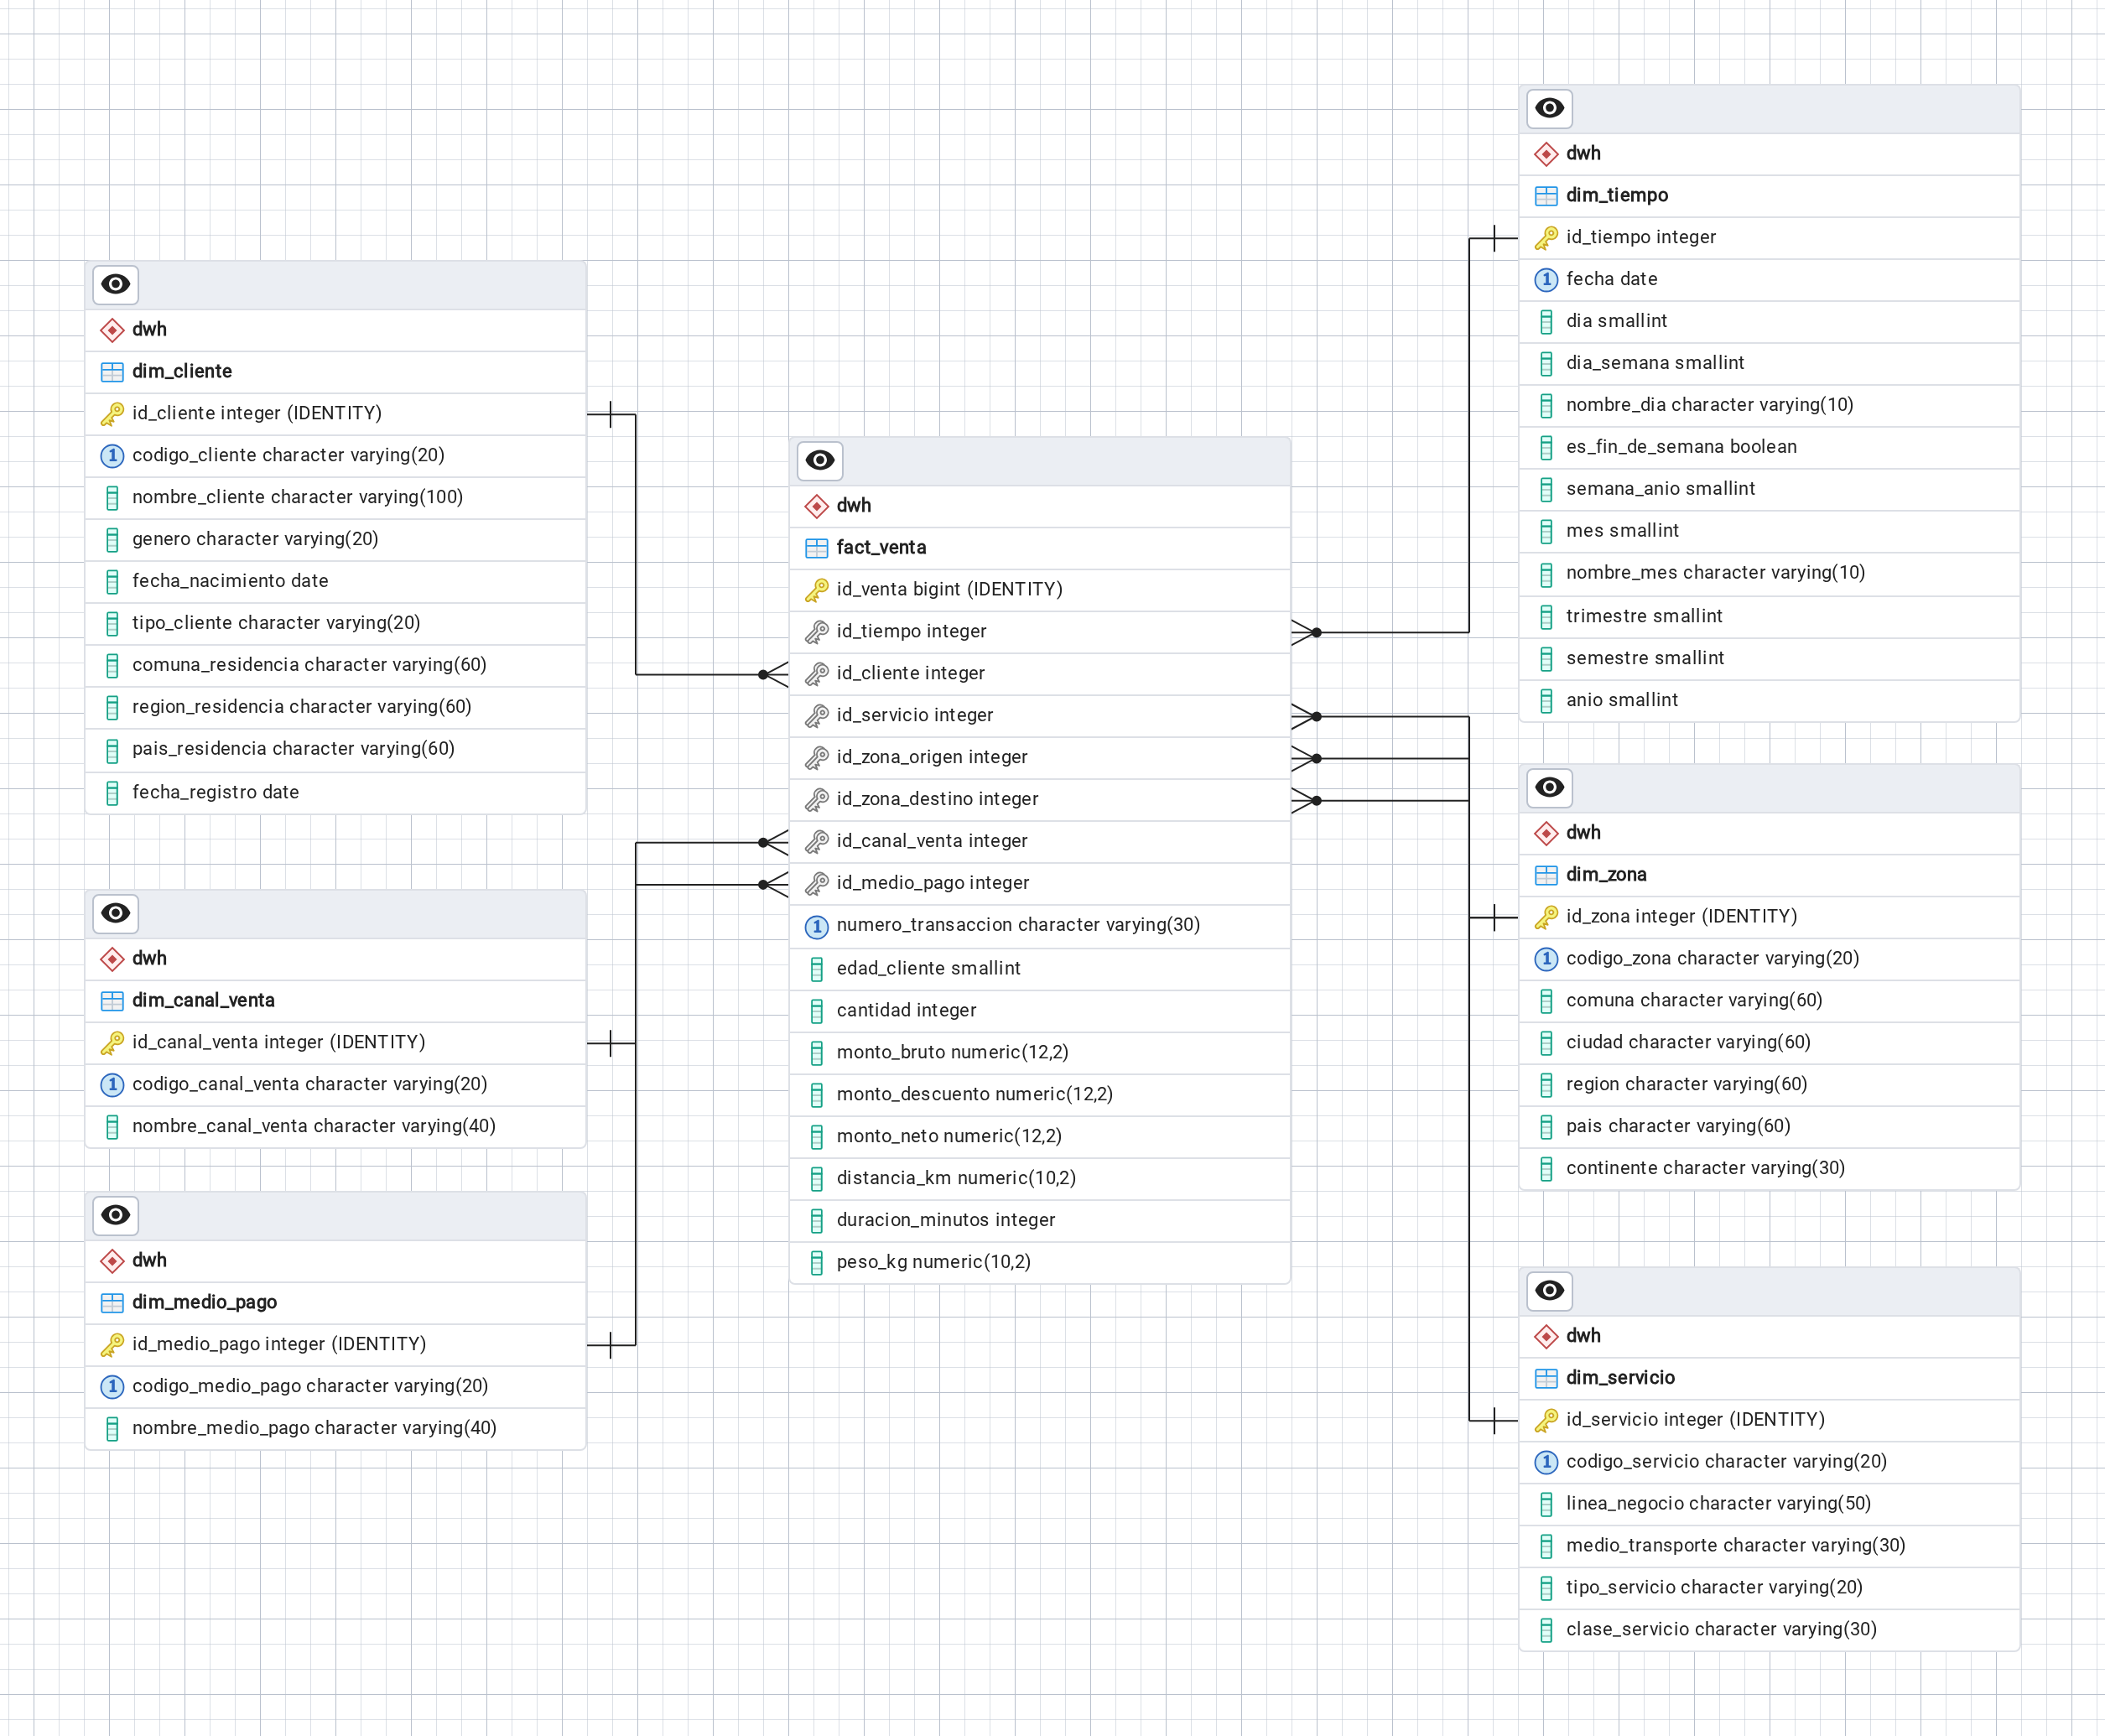
\includegraphics[width=\linewidth,height=0.5\textheight,keepaspectratio]{../docs/diagramas/esquema_estrella.png}%
  }{%
    \fbox{\parbox{0.8\linewidth}{\centering\vspace{3em}%
      Esquema pendiente: \bd{docs/diagramas/esquema_estrella.png}\vspace{3em}}}%
  }
  \caption{Modelo multidimensional estrella de \bd{dwh_rapiditos} (Diseñador de phpMyAdmin)}
  \label{fig:esquema}
\end{figure}

\subsection{Dimensiones}

Todas las dimensiones tienen una llave sustituta autoincremental
(\bd{id_<entidad>}) y una llave natural única (\bd{codigo_<entidad>}). La
excepción es \bd{dim_tiempo}, cuya llave es la fecha en formato AAAAMMDD.

\begin{table}[H]
  \centering
  \caption{Dimensiones del modelo}
  \label{tab:dimensiones}
  \small
  \begin{tabularx}{\linewidth}{@{}l>{\raggedright\arraybackslash}X>{\raggedright\arraybackslash}X@{}}
    \toprule
    \textbf{Dimensión} & \textbf{Propósito} & \textbf{Atributos} \\
    \midrule
    \bd{dim_tiempo} & Análisis anual y por período. Jerarquía fecha, mes,
      trimestre, semestre y año.
      & fecha, día, día de la semana, fin de semana, semana del año, mes,
        trimestre, semestre, año \\
    \bd{dim_cliente} & Vista única del cliente entre las seis líneas.
      & código, nombre, género, fecha de nacimiento, tipo (persona o
        empresa), comuna, región y país de residencia, fecha de registro \\
    \bd{dim_servicio} & Línea de negocio y medio de transporte, en una sola
      tabla para mantener la estrella.
      & código, línea de negocio, medio de transporte, tipo de servicio
        (pasajeros o carga), clase de servicio \\
    \bd{dim_zona} & Zona geográfica, con rol de origen y de destino.
      Jerarquía comuna, ciudad, región, país y continente.
      & código, comuna, ciudad, región, país, continente \\
    \bd{dim_canal_venta} & Canal por el que se realizó la compra.
      & código, nombre del canal (app, web, boletería, call center, convenio
        empresa) \\
    \bd{dim_medio_pago} & Medio de pago de la compra.
      & código, nombre del medio de pago (efectivo, débito, crédito,
        transferencia, billetera digital) \\
    \bottomrule
  \end{tabularx}
\end{table}

\subsection{Tabla de hechos}

La tabla \bd{fact_venta} contiene siete llaves foráneas hacia las
dimensiones, una dimensión degenerada y las medidas de la
Tabla~\ref{tab:medidas}.

\begin{itemize}[leftmargin=*]
  \item \textbf{Llaves foráneas:} \bd{id_tiempo}, \bd{id_cliente},
        \bd{id_servicio}, \bd{id_zona_origen}, \bd{id_zona_destino},
        \bd{id_canal_venta} e \bd{id_medio_pago}.
  \item \textbf{Dimensión degenerada:} \bd{numero_transaccion}, el
        identificador del sistema de origen, prefijado por línea de negocio.
\end{itemize}

\begin{table}[H]
  \centering
  \caption{Medidas de \bd{fact_venta}}
  \label{tab:medidas}
  \small
  \begin{tabularx}{\linewidth}{@{}lll>{\raggedright\arraybackslash}X@{}}
    \toprule
    \textbf{Medida} & \textbf{Tipo de dato} & \textbf{Tipo de medida} & \textbf{Descripción} \\
    \midrule
    \bd{cantidad}         & INT UNSIGNED     & Aditiva    & Pasajes, bultos o unidades \\
    \bd{monto_bruto}      & DECIMAL(12,2)    & Aditiva    & Monto antes de descuento (CLP) \\
    \bd{monto_descuento}  & DECIMAL(12,2)    & Aditiva    & Descuento aplicado (CLP) \\
    \bd{monto_neto}       & DECIMAL(12,2)    & Aditiva    & Monto pagado (CLP) \\
    \bd{distancia_km}     & DECIMAL(10,2)    & Aditiva    & Distancia recorrida \\
    \bd{duracion_minutos} & INT UNSIGNED     & Aditiva    & Duración del servicio \\
    \bd{peso_kg}          & DECIMAL(10,2)    & Aditiva    & Solo logística y delivery \\
    \bd{edad_cliente}     & TINYINT UNSIGNED & No aditiva & Edad al momento de la compra \\
    \bottomrule
  \end{tabularx}
\end{table}

\subsection{Cálculos y KPI derivados}

\begin{table}[H]
  \centering
  \caption{Cálculos y KPI derivados de las medidas}
  \label{tab:kpi}
  \small
  \begin{tabularx}{\linewidth}{@{}l>{\raggedright\arraybackslash}X@{}}
    \toprule
    \textbf{KPI} & \textbf{Cálculo} \\
    \midrule
    Ventas netas              & \bd{SUM(monto_neto)} \\
    Ticket promedio           & \bd{SUM(monto_neto) / COUNT(id_venta)} \\
    Clientes activos por año  & \bd{COUNT(DISTINCT id_cliente)} por año \\
    Frecuencia de compra      & \bd{COUNT(id_venta) / COUNT(DISTINCT id_cliente)} \\
    Gasto anual por cliente   & \bd{SUM(monto_neto) / COUNT(DISTINCT id_cliente)} por año \\
    Participación por línea   & \bd{SUM(monto_neto)} de la línea / \bd{SUM(monto_neto)} total \\
    Clientes multilínea       & Clientes con \bd{COUNT(DISTINCT linea_negocio) > 1} por año \\
    Tasa de descuento         & \bd{SUM(monto_descuento) / SUM(monto_bruto)} \\
    \bottomrule
  \end{tabularx}
\end{table}

\subsection{Norma de nomenclatura}

\begin{itemize}[leftmargin=*]
  \item Prefijo \bd{fact_} para la tabla de hechos y \bd{dim_} para las
        dimensiones.
  \item Nombres en singular, en \bd{snake_case} y en minúsculas, en todas las
        tablas y columnas.
  \item Llave primaria \bd{id_<entidad>} y llave natural \bd{codigo_<entidad>}.
  \item Llave foránea con el mismo nombre que la llave primaria referenciada;
        en la dimensión de rol se agrega un sufijo (\bd{id_zona_origen},
        \bd{id_zona_destino}).
  \item Restricciones con nombre: \bd{fk_<tabla>_<columna>} y
        \bd{uq_<tabla>_<columna>}. La llave primaria se declara sin nombre,
        porque MariaDB la registra siempre como \bd{PRIMARY}.
\end{itemize}

\subsection{Implementación en MariaDB}

El script \bd{sql/01_ddl.sql} crea la base \bd{dwh_rapiditos} con las seis
dimensiones y la tabla de hechos, sin datos. Es idempotente: elimina y vuelve
a crear la base, por lo que se puede ejecutar de corrido en la pestaña SQL de
phpMyAdmin las veces que sea necesario. Todas las tablas usan el motor InnoDB
y el juego de caracteres \bd{utf8mb4}. El script \bd{sql/99_validacion.sql}
consulta \bd{information_schema} para verificar tablas, columnas y llaves.

\captura{01_xampp_activo.png}{XAMPP con Apache y MySQL (MariaDB) activos}
\captura{02_phpmyadmin_ddl_ejecutado.png}{Ejecución de \bd{sql/01_ddl.sql} en la pestaña SQL de phpMyAdmin}
\captura{03_estructura_fact_venta.png}{Estructura de la tabla de hechos \bd{fact_venta} en phpMyAdmin}
\captura{04_disenador_esquema_estrella.png}{Esquema estrella en el Diseñador de phpMyAdmin}
La Figura~\ref{fig:val_tablas} confirma que las siete tablas usan InnoDB y
\bd{utf8mb4_unicode_ci}. La Figura~\ref{fig:val_fk} muestra las siete llaves
foráneas de \bd{fact_venta}, todas con nombre normado. La
Figura~\ref{fig:val_resumen} confirma la estrella: solo la tabla de hechos
tiene llaves foráneas salientes, y \bd{dim_zona} es referenciada dos veces
(origen y destino). Las tres figuras son recortes de la misma ejecución de
\bd{sql/99_validacion.sql}.

\captura[0.65\linewidth]{05a_validacion_tablas.png}{\bd{sql/99_validacion.sql}: tablas, motor y cotejamiento\label{fig:val_tablas}}
\captura{05b_validacion_fk.png}{\bd{sql/99_validacion.sql}: llaves foráneas de la tabla de hechos\label{fig:val_fk}}
\captura[0.56\linewidth]{05c_validacion_resumen.png}{\bd{sql/99_validacion.sql}: resumen de columnas y llaves por tabla\label{fig:val_resumen}}

\clearpage
% =============================================================================
% Capítulo 5: Scripts del Datawarehouse
% Entregable 2 del Avance N°1: script SQL de creación del modelo multidimensional.
% Las cifras de la Tabla de verificación se obtuvieron del catálogo de
% PostgreSQL el 05-11-2026 (ver docs/bitacora.md).
% =============================================================================
\section{Scripts del Datawarehouse}
\label{sec:scripts}

Este capítulo presenta los scripts que crean y verifican el Datawarehouse. En
el Avance N°1 el script crea la estructura del modelo multidimensional
\emph{sin datos}; los scripts de carga se agregan en el Avance N°2.

\subsection{Scripts Entregados}

\begin{table}[H]
  \centering
  \caption{Scripts del Datawarehouse y de apoyo}
  \label{tab:scripts}
  \small
  \begin{tabularx}{\linewidth}{@{}>{\raggedright\arraybackslash}p{5.4cm}
                                  >{\raggedright\arraybackslash}X@{}}
    \toprule
    \textbf{Archivo} & \textbf{Propósito} \\
    \midrule
    \bd{sql/01_ddl.sql} & Crea el esquema \bd{dwh} con las seis dimensiones,
      la tabla de hechos, sus restricciones, índices y comentarios \\
    \bd{sql/99_validacion.sql} & Consulta el catálogo de PostgreSQL para
      verificar tablas, columnas, llaves, restricciones, índices y
      nomenclatura \\
    \bd{tests/test_ddl.py} & 29 pruebas automáticas (pytest) que crean una
      base de prueba, ejecutan el script dos veces y comparan el resultado con
      el diseño \\
    \bd{docker-compose.yml} & Define los servicios PostgreSQL 17 y pgAdmin 4 \\
    \bd{herramientas/capturar_pgadmin.py} & Ejecuta el script y la validación
      en pgAdmin y toma las capturas del informe (Playwright) \\
    \bd{herramientas/generar_diccionario.py} & Genera el diccionario de datos
      del Anexo~A desde el catálogo de la base \\
    \bottomrule
  \end{tabularx}
\end{table}

\subsection{Script de Creación del Modelo}

El script \bd{sql/01_ddl.sql} está escrito para PostgreSQL 17 y se ejecuta de
corrido, sin intervención, tanto con \bd{psql} como en el Query Tool de
pgAdmin. Su estructura es la siguiente:

\begin{enumerate}[leftmargin=*]
  \item \textbf{Codificación:} \bd{SET client_encoding = 'UTF8'}. El archivo
        está en UTF-8, y esta línea asegura que las tildes de los comentarios
        y de las reglas se guarden bien aunque el script se ejecute con
        \bd{psql} desde una consola de Windows, que usa otra codificación.
  \item \textbf{Inicio de la transacción:} \bd{BEGIN}, seguido de
        \bd{DROP SCHEMA IF EXISTS dwh CASCADE} y \bd{CREATE SCHEMA dwh}. El
        script es \emph{idempotente}: se puede ejecutar las veces que sea
        necesario y siempre deja el mismo resultado.
  \item \textbf{Dimensiones:} las seis tablas \bd{dim_}, cada una con su llave
        primaria, su llave natural única y sus reglas \bd{CHECK}.
  \item \textbf{Tabla de hechos:} \bd{fact_venta}, con sus siete llaves
        foráneas (reglas \bd{ON DELETE RESTRICT} y \bd{ON UPDATE RESTRICT}) y
        las reglas de sus medidas.
  \item \textbf{Comentarios:} \bd{COMMENT ON} en el esquema, las 7 tablas y
        las 58 columnas (66 comentarios), que documentan el modelo dentro de la
        propia base.
  \item \textbf{Índices:} uno por cada llave foránea de \bd{fact_venta}, porque
        PostgreSQL no los crea por su cuenta y aceleran los cruces con las
        dimensiones.
  \item \textbf{Fin de la transacción:} \bd{COMMIT}. Si cualquier sentencia
        falla, la transacción se revierte completa y no queda nada a medias.
\end{enumerate}

La Figura~\ref{fig:ddl_fact} muestra la creación de la tabla de hechos. El
script completo se entrega en el repositorio del proyecto.

\begin{figure}[H]
  \centering
  \caption{Fragmento de \bd{sql/01_ddl.sql}: creación de la tabla de hechos \bd{fact_venta}}
  \label{fig:ddl_fact}
  \sinunicode{\lstinputlisting[style=sql, firstline=212, lastline=255,
                   firstnumber=212]{../sql/01_ddl.sql}}
\end{figure}

La Figura~\ref{fig:ddl_ejecutado} muestra la ejecución del script en el Query
Tool de pgAdmin, y la Figura~\ref{fig:estructura_fact} la estructura de la
tabla de hechos resultante.

\captura{02_pgadmin_ddl_ejecutado.png}{Ejecución de \bd{sql/01_ddl.sql} en el Query Tool de pgAdmin\label{fig:ddl_ejecutado}}
\captura{03_estructura_fact_venta.png}{Estructura de la tabla de hechos \bd{fact_venta} en pgAdmin\label{fig:estructura_fact}}

\subsection{Reglas de Integridad}

Además de las llaves, el script declara 20 restricciones \bd{CHECK} que la
base de datos hace cumplir en cada carga. Así, el ETL no puede dejar datos
inconsistentes en el Datawarehouse:

\begin{itemize}[leftmargin=*]
  \item \textbf{Montos:} el monto neto es igual al bruto menos el descuento, y
        el descuento está entre cero y el monto bruto.
  \item \textbf{Medidas no negativas:} la cantidad es de al menos una unidad;
        distancia, duración y peso no pueden ser negativos, y la edad del
        cliente está entre 0 y 120 años.
  \item \textbf{Dimensión tiempo:} la llave AAAAMMDD y cada atributo derivado
        (día, día de la semana, fin de semana, semana del año, mes, trimestre,
        semestre y año) deben coincidir con la fecha.
  \item \textbf{Dominios cerrados:} el tipo de cliente (persona o empresa), el
        tipo de servicio (pasajeros o carga) y la línea de negocio, que solo
        acepta los seis nombres del enunciado.
\end{itemize}

\subsection{Entorno de Ejecución}

El Datawarehouse corre en PostgreSQL 17.11 dentro de un contenedor Docker,
junto con pgAdmin 4 (Figura~\ref{fig:docker}). El esquema estrella creado por
el script se visualiza en el ERD Tool de pgAdmin
(Figura~\ref{fig:erd}).

\captura{01_docker_servicios_activos.png}{Salida de \bd{docker compose ps}: PostgreSQL 17 y pgAdmin activos\label{fig:docker}}
\captura{04_erd_esquema_estrella.png}{Esquema estrella en el ERD Tool de pgAdmin\label{fig:erd}}

\subsection{Verificación del Datawarehouse}
\label{sec:verificacion}

El resultado del script se verificó de tres formas: con las consultas de
\bd{sql/99_validacion.sql}, con las 29 pruebas automáticas de
\bd{tests/test_ddl.py} y ejecutando el script dos veces seguidas, para
comprobar que es idempotente. La Tabla~\ref{tab:verificacion} resume los
elementos del esquema \bd{dwh} consultados en el catálogo de PostgreSQL.

\begin{table}[H]
  \centering
  \caption{Elementos del esquema \bd{dwh} verificados en el catálogo}
  \label{tab:verificacion}
  \small
  \begin{tabularx}{\linewidth}{@{}>{\raggedright\arraybackslash}X cc@{}}
    \toprule
    \textbf{Elemento} & \textbf{Esperado según el diseño} & \textbf{Obtenido} \\
    \midrule
    Tablas (1 de hechos y 6 dimensiones)    & 7  & 7  \\
    Columnas                                & 58 & 58 \\
    Llaves primarias                        & 7  & 7  \\
    Restricciones \bd{UNIQUE}               & 7  & 7  \\
    Llaves foráneas (todas en \bd{fact_venta}) & 7  & 7  \\
    Restricciones \bd{CHECK}                & 20 & 20 \\
    Índices sobre llaves foráneas           & 7  & 7  \\
    Comentarios (esquema, tablas y columnas) & 66 & 66 \\
    Restricciones o índices fuera de la norma de nomenclatura & 0 & 0 \\
    Filas cargadas (Avance N°1, sin datos)  & 0  & 0  \\
    \bottomrule
  \end{tabularx}
  \nota{Consultas ejecutadas en PostgreSQL 17.11 el 05-11-2026.}
\end{table}

Las pruebas automáticas crean una base de prueba aparte, ejecutan el script
dos veces y comparan la base resultante con el diseño de
\bd{docs/modelo_dimensional.md}: tablas, columnas, tipos, llaves, reglas e
índices. También intentan insertar datos inválidos, como un monto neto que no
cuadra con el bruto o una venta con un cliente inexistente, y comprueban que la
base los rechaza. Las 29 pruebas se aprobaron.

Las figuras siguientes son resultados de \bd{sql/99_validacion.sql}. La
Figura~\ref{fig:val_tablas} muestra las siete tablas del esquema con su
comentario. La Figura~\ref{fig:val_fk} muestra las siete llaves foráneas de
\bd{fact_venta}, todas con nombre normado y regla \bd{RESTRICT}. La
Figura~\ref{fig:val_resumen} confirma la estrella: solo la tabla de hechos
tiene llaves foráneas salientes, y \bd{dim_zona} es referenciada dos veces
(origen y destino). La Figura~\ref{fig:val_checks} lista las reglas de
integridad, y la Figura~\ref{fig:val_nomenclatura} muestra que ninguna
restricción ni índice queda fuera de la norma de nomenclatura.

\captura{05a_validacion_tablas.png}{\bd{sql/99_validacion.sql}: tablas del esquema \bd{dwh}\label{fig:val_tablas}}
\captura{05b_validacion_fk.png}{\bd{sql/99_validacion.sql}: llaves foráneas de la tabla de hechos\label{fig:val_fk}}
\captura{05c_validacion_resumen.png}{\bd{sql/99_validacion.sql}: resumen de columnas y llaves por tabla\label{fig:val_resumen}}
\captura{05d_validacion_checks.png}{\bd{sql/99_validacion.sql}: restricciones \bd{CHECK}\label{fig:val_checks}}
\captura{05e_validacion_nomenclatura.png}{\bd{sql/99_validacion.sql}: control de nomenclatura (0 filas fuera de norma)\label{fig:val_nomenclatura}}

\clearpage
% =============================================================================
% Capítulo 6: Bibliografía
% Las referencias están en informe/referencias.bib y las procesa BibTeX con el
% estilo babunsrt (babelbib): numeradas en orden de aparición y en español.
% =============================================================================
\section{Bibliografía}
\label{sec:bibliografia}

% thebibliography crea su propio \section*; se anula dentro del grupo para que
% el capítulo quede numerado en el índice.
\begingroup
\renewcommand{\section}[2]{}
\raggedright
\bibliographystyle{babunsrt}
\bibliography{referencias}
\endgroup

\clearpage
% =============================================================================
% Capítulo 7: Anexos
% =============================================================================
\section{Anexos}
\label{sec:anexos}

\subsection{Anexo A: Diccionario de Datos}
\label{sec:anexo_diccionario}

Este anexo describe cada columna del esquema \bd{dwh}: tipo de dato, si admite
nulos, las llaves y reglas en que participa (PK: llave primaria; FK: llave
foránea; UQ: valor único; CK: regla \bd{CHECK}) y su descripción. Las
descripciones son los comentarios \bd{COMMENT ON} del propio script, y el
anexo se genera desde el catálogo de PostgreSQL con
\bd{herramientas/generar_diccionario.py}, por lo que coincide con la base
creada.

% =============================================================================
% Anexo A: Diccionario de Datos.
% Generado por herramientas/generar_diccionario.py desde el catálogo de
% PostgreSQL. No editar a mano: volver a ejecutar el script.
% =============================================================================

\subsubsection{Tabla \bd{fact_venta}}

Hechos de venta: una fila por transacción de compra de un cliente. \textbf{Origen:} Transacciones de las seis fuentes públicas de la Sección~\ref{sec:fuentes} (una fila por pasaje, viaje, envío o pedido), asignadas a clientes sintéticos.

\begin{table}[H]
  \centering
  \caption{Diccionario de datos de \bd{fact_venta}}
  \small
  \begin{tabularx}{\linewidth}{@{}>{\raggedright\arraybackslash}p{4.0cm}lcl>{\raggedright\arraybackslash}X@{}}
    \toprule
    \textbf{Columna} & \textbf{Tipo} & \textbf{Nulo} & \textbf{Clave} & \textbf{Descripción} \\
    \midrule
    \bd{id_venta} & BIGINT & No & PK & PK. Llave sustituta \\
    \bd{id_tiempo} & INTEGER & No & FK & FK a dim\_tiempo (fecha de la compra) \\
    \bd{id_cliente} & INTEGER & No & FK & FK a dim\_cliente \\
    \bd{id_servicio} & INTEGER & No & FK & FK a dim\_servicio \\
    \bd{id_zona_origen} & INTEGER & No & FK & FK a dim\_zona, rol origen \\
    \bd{id_zona_destino} & INTEGER & No & FK & FK a dim\_zona, rol destino \\
    \bd{id_canal_venta} & INTEGER & No & FK & FK a dim\_canal\_venta \\
    \bd{id_medio_pago} & INTEGER & No & FK & FK a dim\_medio\_pago \\
    \bd{numero_transaccion} & VARCHAR(30) & No & UQ & Dimensión degenerada: id del sistema de origen, prefijado por línea \\
    \bd{edad_cliente} & SMALLINT & Sí & CK & Edad al momento de la compra (no aditiva; NULL para empresas) \\
    \bd{cantidad} & INTEGER & No & CK & Medida aditiva: pasajes, bultos o unidades \\
    \bd{monto_bruto} & NUMERIC(12,2) & No & CK & Medida aditiva: monto antes de descuento (CLP) \\
    \bd{monto_descuento} & NUMERIC(12,2) & No & CK & Medida aditiva: descuento aplicado (CLP) \\
    \bd{monto_neto} & NUMERIC(12,2) & No & CK & Medida aditiva: monto pagado (CLP) = bruto - descuento \\
    \bd{distancia_km} & NUMERIC(10,2) & Sí & CK & Medida aditiva: distancia recorrida en km \\
    \bd{duracion_minutos} & INTEGER & Sí & CK & Medida aditiva: duración del servicio en minutos \\
    \bd{peso_kg} & NUMERIC(10,2) & Sí & CK & Medida aditiva: peso en kg (solo logística y delivery) \\
    \bottomrule
  \end{tabularx}
\end{table}

\subsubsection{Tabla \bd{dim_tiempo}}

Dimensión tiempo con granularidad diaria. \textbf{Origen:} Se genera con un script SQL (\bd{generate_series}) para 2023 a 2025; no requiere fuente externa.

\begin{table}[H]
  \centering
  \caption{Diccionario de datos de \bd{dim_tiempo}}
  \small
  \begin{tabularx}{\linewidth}{@{}>{\raggedright\arraybackslash}p{4.0cm}lcl>{\raggedright\arraybackslash}X@{}}
    \toprule
    \textbf{Columna} & \textbf{Tipo} & \textbf{Nulo} & \textbf{Clave} & \textbf{Descripción} \\
    \midrule
    \bd{id_tiempo} & INTEGER & No & PK, CK & PK. Fecha en formato AAAAMMDD (ej. 20250314) \\
    \bd{fecha} & DATE & No & UQ & Fecha calendario \\
    \bd{dia} & SMALLINT & No & CK & Día del mes (1-31) \\
    \bd{dia_semana} & SMALLINT & No & CK & 1 = lunes … 7 = domingo (ISO) \\
    \bd{nombre_dia} & VARCHAR(10) & No &  & Lunes … Domingo \\
    \bd{es_fin_de_semana} & BOOLEAN & No & CK & TRUE si es sábado o domingo \\
    \bd{semana_anio} & SMALLINT & No & CK & Semana ISO del año (1-53) \\
    \bd{mes} & SMALLINT & No & CK & Mes (1-12) \\
    \bd{nombre_mes} & VARCHAR(10) & No &  & Enero … Diciembre \\
    \bd{trimestre} & SMALLINT & No & CK & Trimestre (1-4) \\
    \bd{semestre} & SMALLINT & No & CK & Semestre (1-2) \\
    \bd{anio} & SMALLINT & No & CK & Año \\
    \bottomrule
  \end{tabularx}
\end{table}

\subsubsection{Tabla \bd{dim_cliente}}

Dimensión cliente unificada entre las seis líneas de negocio. \textbf{Origen:} Sintética: clientes residentes en Chile, con la distribución por comuna, sexo y edad del Censo de Población y Vivienda 2024.

\begin{table}[H]
  \centering
  \caption{Diccionario de datos de \bd{dim_cliente}}
  \small
  \begin{tabularx}{\linewidth}{@{}>{\raggedright\arraybackslash}p{4.0cm}lcl>{\raggedright\arraybackslash}X@{}}
    \toprule
    \textbf{Columna} & \textbf{Tipo} & \textbf{Nulo} & \textbf{Clave} & \textbf{Descripción} \\
    \midrule
    \bd{id_cliente} & INTEGER & No & PK & PK. Llave sustituta \\
    \bd{codigo_cliente} & VARCHAR(20) & No & UQ & Llave natural (RUT o documento, unificado entre líneas) \\
    \bd{nombre_cliente} & VARCHAR(100) & No &  & Nombre o razón social \\
    \bd{genero} & VARCHAR(20) & Sí &  & Género declarado (NULL para empresas) \\
    \bd{fecha_nacimiento} & DATE & Sí &  & Fecha de nacimiento (NULL para empresas) \\
    \bd{tipo_cliente} & VARCHAR(20) & No & CK & persona o empresa \\
    \bd{comuna_residencia} & VARCHAR(60) & Sí &  & Comuna de residencia \\
    \bd{region_residencia} & VARCHAR(60) & Sí &  & Región de residencia \\
    \bd{pais_residencia} & VARCHAR(60) & No &  & País de residencia \\
    \bd{fecha_registro} & DATE & Sí &  & Fecha de alta como cliente \\
    \bottomrule
  \end{tabularx}
\end{table}

\subsubsection{Tabla \bd{dim_servicio}}

Dimensión servicio: línea de negocio y medio de transporte. \textbf{Origen:} Catálogo de los servicios de cada línea de negocio, con los atributos que informa cada fuente (tipo y clase de servicio, medio de transporte).

\begin{table}[H]
  \centering
  \caption{Diccionario de datos de \bd{dim_servicio}}
  \small
  \begin{tabularx}{\linewidth}{@{}>{\raggedright\arraybackslash}p{4.0cm}lcl>{\raggedright\arraybackslash}X@{}}
    \toprule
    \textbf{Columna} & \textbf{Tipo} & \textbf{Nulo} & \textbf{Clave} & \textbf{Descripción} \\
    \midrule
    \bd{id_servicio} & INTEGER & No & PK & PK. Llave sustituta \\
    \bd{codigo_servicio} & VARCHAR(20) & No & UQ & Llave natural \\
    \bd{linea_negocio} & VARCHAR(50) & No & CK & Una de las 6 líneas de negocio del enunciado (nombre literal) \\
    \bd{medio_transporte} & VARCHAR(30) & No &  & bus, tren, taxi, camión, avión, moto/bicicleta \\
    \bd{tipo_servicio} & VARCHAR(20) & No & CK & pasajeros o carga \\
    \bd{clase_servicio} & VARCHAR(30) & No &  & Ej. económica, ejecutiva, express, estándar \\
    \bottomrule
  \end{tabularx}
\end{table}

\subsubsection{Tabla \bd{dim_zona}}

Dimensión zona geográfica, de rol doble (origen y destino). \textbf{Origen:} Tablas de zonas de cada fuente (zonas de taxi de Nueva York, puntos de ANTT, estaciones del Reino Unido, aeropuertos de EE.UU.) y comunas de Chile del Censo 2024.

\begin{table}[H]
  \centering
  \caption{Diccionario de datos de \bd{dim_zona}}
  \small
  \begin{tabularx}{\linewidth}{@{}>{\raggedright\arraybackslash}p{4.0cm}lcl>{\raggedright\arraybackslash}X@{}}
    \toprule
    \textbf{Columna} & \textbf{Tipo} & \textbf{Nulo} & \textbf{Clave} & \textbf{Descripción} \\
    \midrule
    \bd{id_zona} & INTEGER & No & PK & PK. Llave sustituta \\
    \bd{codigo_zona} & VARCHAR(20) & No & UQ & Llave natural \\
    \bd{comuna} & VARCHAR(60) & No &  & Comuna (No aplica en destinos internacionales) \\
    \bd{ciudad} & VARCHAR(60) & No &  & Ciudad \\
    \bd{region} & VARCHAR(60) & No &  & Región \\
    \bd{pais} & VARCHAR(60) & No &  & País \\
    \bd{continente} & VARCHAR(30) & No &  & Continente \\
    \bottomrule
  \end{tabularx}
\end{table}

\subsubsection{Tabla \bd{dim_canal_venta}}

Dimensión canal de venta. \textbf{Origen:} Canales de compra informados por las fuentes, normalizados a un catálogo común.

\begin{table}[H]
  \centering
  \caption{Diccionario de datos de \bd{dim_canal_venta}}
  \small
  \begin{tabularx}{\linewidth}{@{}>{\raggedright\arraybackslash}p{4.0cm}lcl>{\raggedright\arraybackslash}X@{}}
    \toprule
    \textbf{Columna} & \textbf{Tipo} & \textbf{Nulo} & \textbf{Clave} & \textbf{Descripción} \\
    \midrule
    \bd{id_canal_venta} & INTEGER & No & PK & PK. Llave sustituta \\
    \bd{codigo_canal_venta} & VARCHAR(20) & No & UQ & Llave natural \\
    \bd{nombre_canal_venta} & VARCHAR(40) & No &  & app, web, boletería, call center, convenio empresa \\
    \bottomrule
  \end{tabularx}
\end{table}

\subsubsection{Tabla \bd{dim_medio_pago}}

Dimensión medio de pago. \textbf{Origen:} Tipos de pago informados por las fuentes, normalizados a un catálogo común.

\begin{table}[H]
  \centering
  \caption{Diccionario de datos de \bd{dim_medio_pago}}
  \small
  \begin{tabularx}{\linewidth}{@{}>{\raggedright\arraybackslash}p{4.0cm}lcl>{\raggedright\arraybackslash}X@{}}
    \toprule
    \textbf{Columna} & \textbf{Tipo} & \textbf{Nulo} & \textbf{Clave} & \textbf{Descripción} \\
    \midrule
    \bd{id_medio_pago} & INTEGER & No & PK & PK. Llave sustituta \\
    \bd{codigo_medio_pago} & VARCHAR(20) & No & UQ & Llave natural \\
    \bd{nombre_medio_pago} & VARCHAR(40) & No &  & efectivo, débito, crédito, transferencia, billetera digital \\
    \bottomrule
  \end{tabularx}
\end{table}


\subsection{Anexo B: Reproducción del Entorno}
\label{sec:anexo_entorno}

\subsubsection{Ejecución de los Scripts en Cualquier Equipo}

Los scripts \bd{01_ddl.sql} y \bd{99_validacion.sql} son autónomos: no leen ni
escriben archivos, no dependen de otros archivos y se ejecutan desde cualquier
carpeta, en Windows, Linux o macOS. Solo requieren PostgreSQL 17 y una base de
datos existente; se recomienda una base nueva, porque \bd{01_ddl.sql} borra y
vuelve a crear el esquema \bd{dwh}.

\begin{enumerate}[leftmargin=*]
  \item Crear una base de datos UTF-8, por ejemplo \bd{rapiditos}.
  \item En pgAdmin, abrir \bd{01_ddl.sql} en el Query Tool de esa base y
        ejecutarlo completo con F5. Con \bd{psql}, desde la carpeta en que
        estén los scripts:
\begin{lstlisting}[style=consola]
psql -U <usuario> -d rapiditos -v ON_ERROR_STOP=1 -f 01_ddl.sql
psql -U <usuario> -d rapiditos -P pager=off -f 99_validacion.sql
\end{lstlisting}
  \item Comparar el resultado de \bd{99_validacion.sql} con la
        Tabla~\ref{tab:verificacion}: la última consulta debe devolver cero
        filas.
\end{enumerate}

Para Windows se entrega además la guía \bd{guia_ejecucion_windows.pdf}, que
detalla paso a paso la instalación de PostgreSQL y pgAdmin, la ejecución con
\bd{psql} y una alternativa con Docker Desktop que no requiere instalar
PostgreSQL ni ningún otro archivo del proyecto.

\subsubsection{Entorno de Desarrollo del Grupo}

El grupo trabaja con el repositorio completo del proyecto, que define
PostgreSQL y pgAdmin en \bd{docker-compose.yml} e incluye las pruebas
automáticas. Estos pasos requieren ese repositorio y se ejecutan desde su
raíz, igual en Linux y en Windows; solo cambian la copia del archivo
\bd{.env} y la activación del entorno virtual de Python, indicadas en los
comentarios.

\begin{enumerate}[leftmargin=*]
  \item Preparar las credenciales y levantar PostgreSQL y pgAdmin. En
        \bd{.env} se definen las contraseñas de ambos servicios.
\begin{lstlisting}[style=consola]
cp .env.example .env      # Windows: copy .env.example .env
docker compose up -d
docker compose ps         # ambos servicios deben aparecer activos
\end{lstlisting}
  \item Crear el modelo multidimensional; pgAdmin queda en
        \bd{http://localhost:5050}.
\begin{lstlisting}[style=consola]
docker compose exec postgres psql -U rapiditos -d rapiditos \
    -v ON_ERROR_STOP=1 -f /sql/01_ddl.sql
\end{lstlisting}
  \item Crear el entorno de Python y ejecutar las pruebas automáticas, que
        usan una base de prueba aparte y nunca modifican \bd{rapiditos}.
\begin{lstlisting}[style=consola]
python -m venv .venv
source .venv/bin/activate # Windows: .venv\Scripts\activate
pip install -r requirements.txt
pytest -v
\end{lstlisting}
  \item Opcionalmente, regenerar el diccionario de datos del Anexo~A y las
        capturas del informe.
\begin{lstlisting}[style=consola]
python herramientas/generar_diccionario.py
python -m playwright install chromium   # una sola vez
python herramientas/capturar_pgadmin.py
\end{lstlisting}
\end{enumerate}

\subsection{Anexo C: Repositorio del Proyecto}
\label{sec:anexo_repositorio}

El código fuente completo del proyecto está publicado en un repositorio
público de GitHub:

\begin{center}
  \url{https://github.com/hirojika/datawarehouse-transportes-rapiditos}
\end{center}

El repositorio reúne los scripts del Datawarehouse, las pruebas automáticas,
las herramientas de apoyo, la documentación del diseño y las fuentes de este
informe, de modo que cualquier persona puede revisar o reproducir el trabajo.
Cada entrega se registra en Git con un commit descriptivo, y el archivo
\bd{docs/bitacora.md} documenta, con fecha, cada decisión, cambio y
verificación realizada durante el proyecto. La Tabla~\ref{tab:repositorio}
describe su contenido.

\begin{table}[H]
  \centering
  \caption{Contenido del repositorio del proyecto}
  \label{tab:repositorio}
  \small
  \begin{tabularx}{\linewidth}{@{}>{\raggedright\arraybackslash}p{4.4cm}
                                  >{\raggedright\arraybackslash}X@{}}
    \toprule
    \textbf{Carpeta o archivo} & \textbf{Contenido} \\
    \midrule
    \bd{sql/} & Scripts del Datawarehouse: \bd{01_ddl.sql} (creación del
      modelo estrella) y \bd{99_validacion.sql} (verificación) \\
    \bd{docs/} & Diseño del modelo dimensional (\bd{modelo_dimensional.md},
      fuente de verdad del diseño), fuentes de información, bitácora,
      diagrama del esquema estrella y capturas del proceso \\
    \bd{informe/} & Fuentes LaTeX de este informe y de la guía de ejecución en
      Windows, con las referencias en \bd{referencias.bib} \\
    \bd{tests/} & Pruebas automáticas del script del Datawarehouse (pytest) \\
    \bd{herramientas/} & Captura automatizada de pgAdmin, generación del
      diccionario de datos (Anexo~A) y armado del paquete de entrega \\
    \bd{docker-compose.yml}, \bd{docker/} & Definición de los servicios
      PostgreSQL 17 y pgAdmin 4, con versiones fijas \\
    \bd{requirements.txt}, \bd{.env.example} & Dependencias de Python con
      versiones fijas y plantilla de configuración de la conexión \\
    \bd{etl/}, \bd{dashboard/}, \bd{data/} & Carpetas reservadas para el
      proyecto de Apache Hop, el dashboard en Streamlit y los datos de origen,
      que se desarrollan en los Avances N°2 y N°3 \\
    \bottomrule
  \end{tabularx}
\end{table}

Por seguridad y derechos de autor, el repositorio no incluye las credenciales
de conexión (archivo \bd{.env}, que cada integrante crea a partir de
\bd{.env.example}) ni el material del curso entregado por el profesor. Para
obtener una copia local se usa:

\begin{lstlisting}[style=consola]
git clone https://github.com/hirojika/datawarehouse-transportes-rapiditos.git
\end{lstlisting}

Los pasos para levantar el entorno a partir de esa copia están en el
Anexo~B (Sección~\ref{sec:anexo_entorno}).


\end{document}
